\begin{center}
  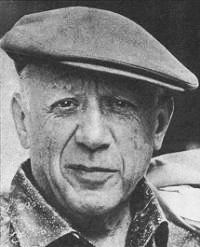
\includegraphics[width=0.55\textwidth]{pablo.jpg}
\end{center}

Pablo Picasso fue un pintor español creador del cubismo. Su padre fue profesor en la academia de bellas artes y ayudò su hijo con la pintura.
Se conoce como periodo azul de picasso al que discurre entre 1901 hasta 1904 y tiene su origen en el suicidio de su amigo que lo dejò lleno de dolor y tristeza.
En el 1905 el pasò de la epoca azul a la denominada epoca rosa que se destinsue por sus colores pastel y tonos càlidos, con lineas delicadas.
Con las señoritas de aviñon como punto de partida Picasso acabò formulando el cubismo.
En el 1937 se produjò el brutal bombardeo de la localidad de Guernica por parte de la Alemania.
Picasso se inspirò en este hecho para la creaciòn de una de sus obras mas famosas.
El cuadro simboliza dodo ul horror de la guerra y la tragedia de la muerte de muchas victimas inocentes.
En 1973 , a la edad de 91 años, muriò en Francia.
